%=======================+==============================
%============    Summary   =============
%======================================================

\section{Summary and outlook\label{sec:summary} }
We have presented the design, construction and performance during the first phase of operation of the  \gx~ experiment in Hall D at Jefferson Lab. 
The experiment operated routinely at an incident photon flux of $2\times 10^{7}$ photons/s in the coherent peak\footnote{Defined as 0.6 GeV below the coherent edge, which varied somewhat depending on the primary incident electron beam energy.} with an open trigger taking data
at 40 kHz and recording 600 MB/s to tape and live time $>$95\%. 
During this time the experiment accumulated  121.4 pb$^{-1}$ in the coherent peak. and 319.4 pb$^{-1}$ for $E_\gamma>$8.1 GeV. We accumulated approximately 270 billion triggers during this period. as shown in Fig.\,\ref{fig:plot_rcdb3_phaseI}.  

\begin{figure}[tbh]\centering
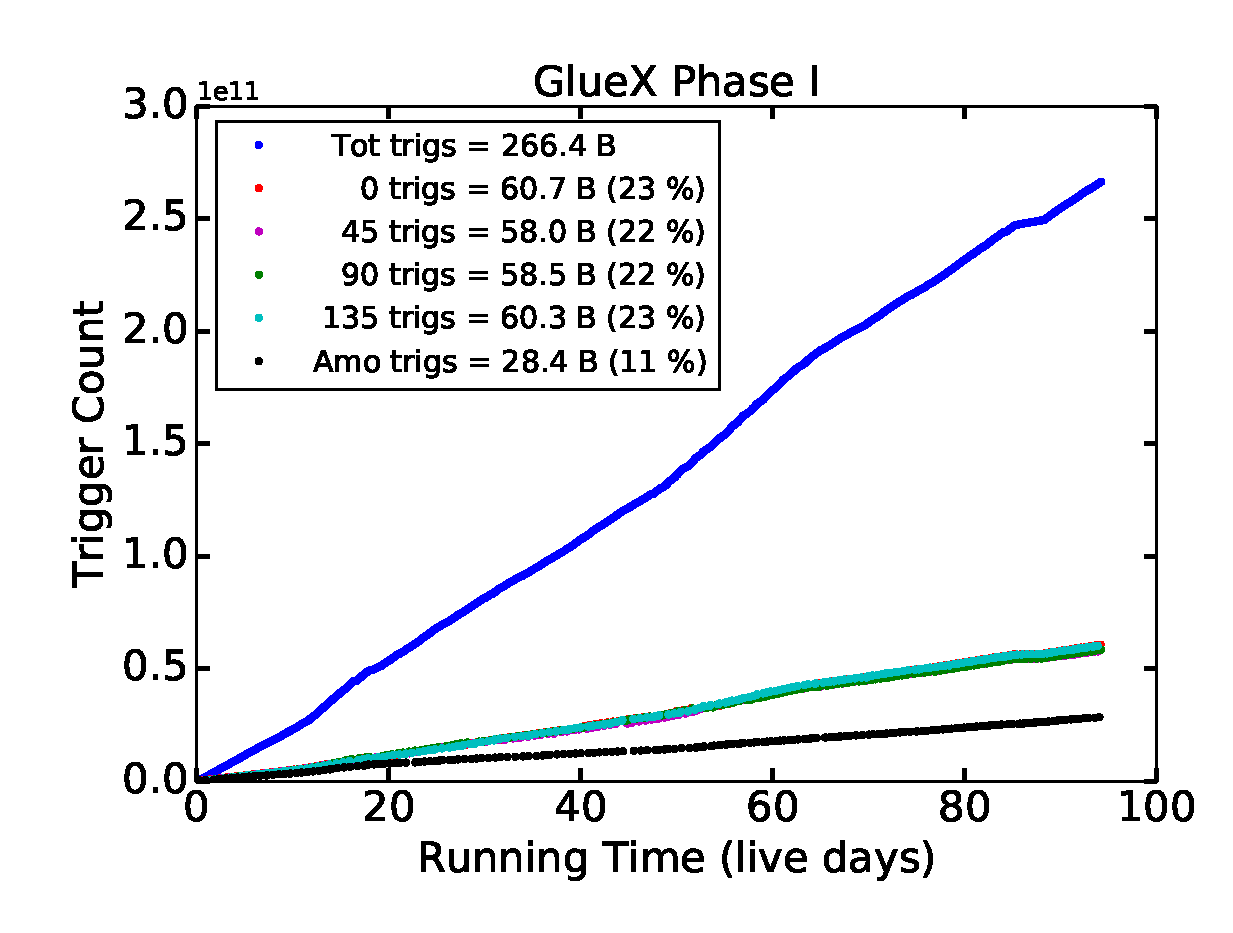
\includegraphics[width=0.48\textwidth]{figures/plot_rcdb3_phaseI.eps}
\caption{\label{fig:plot_rcdb3_phaseI} 
Plot of integrated number of triggers versus the number of live days
in 2016, 2017 and 2018. The triggers of the four diamond configurations fall on top of one another, as we attempted to match the amount of data taken for each configuration. 
(Color online)
 }
\end{figure}   

We have verified the operational characteristics of the charged and neutral particle detector systems and checked that individual systems performed as designed. We have also demonstrated that the detector as a whole is able to reconstruct exclusive final states, determined the reconstruction efficiencies and validated our Monte Carlo simulation against data. The infrastructure is in place to process our high volume of data both on the JLab computing farm as well on other offsite facilities. The use of these tools gives us the ability to process the data in a timely fashion.

Future running will include taking data at higher luminosity  and with improved particle identification capability. 
The \gx~experiment has already implemented the necessary infrastructure to allow us to operate at a flux of $5\times10^{7}$ photons/s in the coherent peak for the upcoming run periods and has added a new DIRC detector\footnote{Four ``bar boxes" from the BaBar \cite{Aubert:2001tu} detector have been installed and tested.} to extend the particle identification of kaons to higher momenta. 

